%--- Kapitel 7
\cleardoublepage
\chapter{Softwarearchitektur und Entwurfsprinzipien}
\label{sec:Kap-7}

Die Festlegung der Softwarearchitektur ist eine zentrale Aufgabe des Software-
\linebreak %%% für Druck
engineering-""Kernprozesses Softwareentwurf. Daran schließt sich die Ausgestaltung der einzelnen Komponenten des Softwaresystems und ihrer Schnittstellen an. Die Themen Software\-architektur auf der einen Seite und Komponenten und Schnittstellen auf der anderen Seite sind eng verbunden. Dieses Kapitel behandelt zunächst das Thema Softwarearchitektur (Kap.~\ref{sec:Kap-7.1}) und anschließend grundlegende Entwurfsprinzipien für Komponenten und Schnittstellen (Kap.~\ref{sec:Kap-7.2}). Die Entwurfsprinzipien lassen sich sowohl auf der Ebene der Softwarearchitektur als auch auf niedrigeren Ebenen von Komponenten und Klassen anwenden und hätten daher auch in das folgende Kapitel~\ref{sec:Kap-8} gepasst. Wir haben sie hier in Kapitel 7 platziert, weil sie mit den im Rahmen der Softwarearchitektur wichtigen Architekturmustern (Kap.~\ref{sec:Kap-7.1.2}) denselben Einsatzzweck teilen: Gute, in der Praxis bewährte Entwürfe für andere zugänglich machen und wiederverwenden.


% 7.1
\clearpage
\section{Softwarearchitektur}
\label{sec:Kap-7.1}

Die Softwarearchitektur beschreibt die Gesamtstruktur eines Softwaresystems. Sie stellt auf einer hohen Abstraktionsebene dar, aus welchen großen Komponenten das System aufgebaut sein soll, wie diese Komponenten zueinander in Beziehung stehen, auf welche Weise sie miteinander interagieren und wie das Gesamtsystem und seine Komponenten mit Elementen außerhalb des Systems interagieren.

\vspace{2mm} %%% für Druck

Eine Komponente ist grundsätzlich eine Einheit zusammengehöriger Funktionalität. \marginline{Komponente} Der Begriff Komponente wird im Rahmen des Softwareentwurfs für sehr unterschiedlich „große“ Teile des Softwareprodukts verwendet. Auf einer niedrigen Abstraktions\-ebene kann man eine Klasse als Komponente des Programms betrachten oder sogar eine Operation als Komponente einer Klasse. Aus der hohen Abstraktions\-sicht der Softwarearchitektur ist eine Komponente ein komplettes Teilstück des Software\-produkts, wie zum Beispiel die Benutzungsschnittstelle, die Datenhaltung, ein Authentifizierungs- oder ein Logging-Mechanismus, das selbst wieder aus kleineren Komponenten zusammengesetzt sein kann.

\vspace{2mm} %%% für Druck

Der Entwurf der Architektur des Softwaresystems ist in der Regel der erste Schritt im Prozess des Softwareentwurfs. Will man die Architektur im späteren Verlauf des Softwareentwicklungsprojekts überarbeiten, ist das meistens teuer, da man sehr viele schon spezifizierte oder sogar schon umgesetzte einzelne Komponenten verändern muss. Eventuell muss man sogar von vorne beginnen.

\vspace{2mm} %%% für Druck

Die für ein Softwaresystem gewählte Architektur hat einen grundlegenden Einfluss darauf, wie sich das System im späteren Einsatz verhält. Ungünstig getroffene architektonische Entscheidungen können Konsequenzen haben, die man schlimmstenfalls erst beim späteren Betrieb des Softwareprodukts bemerkt. Abbildung~\ref{fig:einfluss_architekturentscheidung} zeigt ein eingängiges – wenn auch IT-fernes – Beispiel aus \cite[97]{som20}, bei dem sich eine Architekturentscheidung auf die Systemsicherheit ausgewirkt hat.

\vspace{2mm} %%% für Druck

\begin{figure}[h!]
	\centering
	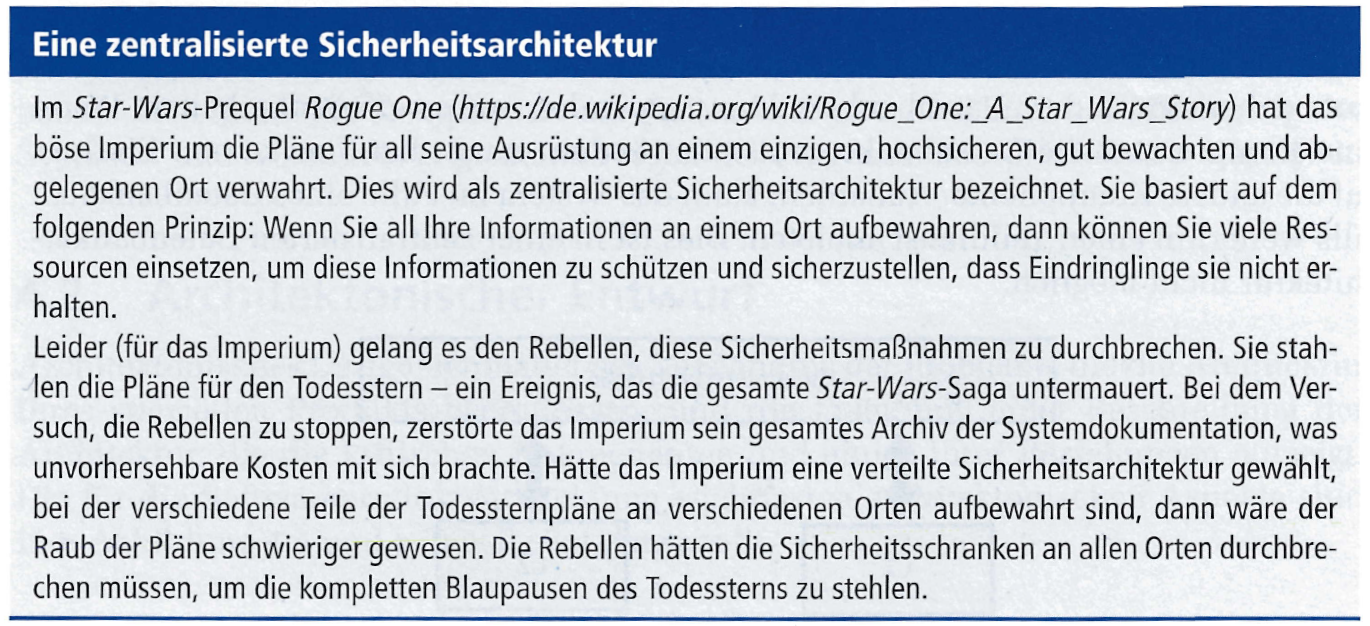
\includegraphics[width=\textwidth]{Bilder/Kapitel-7/einfluss_architekturentscheidung.png}
	\caption[IT-fernes Beispiel für den Einfluss einer Architekturentscheidung auf die Systemeigenschaften]{IT-fernes Beispiel für den Einfluss einer Architekturentscheidung auf die Systemeigenschaften \cite[97]{som20}}
	\label{fig:einfluss_architekturentscheidung}
\end{figure}

\minisec{Architekturen dokumentieren}

Über spezifische Architekturbeschreibungssprachen kann eine Softwarearchitektur sehr formal und sehr detailliert modelliert werden. Auch die UML bietet Diagramme (Komponentendiagramm, Verteilungsdiagramm, eingeschränkt auch Paket-
\linebreak %%% für Druck
diagramm) zur Modellierung der Softwarearchitektur an. Häufig arbeitet man in der Praxis aber mit sehr informellen Diagrammen, zum Beispiel indem Komponenten einfach als (auch ineinander geschachtelte) Kästen gezeichnet und mit Pfeilen zwischen ihnen grob die Beziehungen dargestellt werden. Gerade während der Entstehungszeit der Softwarearchitektur, wenn noch viel mündlich diskutiert wird und Anpassungen vorgenommen werden, ist ein solches informelles Vorgehen sinnvoll, weil es deutlich weniger aufwändig ist. Die Erstellung einer endgültigen „schriftlichen“ Architekturspezifikation als Basis für die Implementierung – manche Projekte verzichten allerdings darauf – oder die Dokumentation einer vorhandenen Architektur erfordert detailliertere Ausdrucksmöglichkeiten als einfache Kästen und Pfeile. Für solche Zwecke muss dann die UML oder eine spezifische Architekturbeschreibungssprache verwendet werden. Dies erfordert die Einarbeitung aller Beteiligten in die gewählte Sprache. Vor allem in agilen Projekten bleibt es zwar häufig bei den informellen Beschreibungen statt einer detaillierteren Ausarbeitung. Die grundsätzlichen Entscheidungen zur Softwarearchitektur müssen allerdings auch dort getroffen werden, auch agile Projekte kommen nicht ohne Architekturentwurf aus.
\subsection{Architektonische Entscheidungen}
\label{sec:Kap-7.1.1}

Die gewählte Softwarearchitektur hat großen Einfluss darauf, wie leistungsfähig und benutzerfreundlich, wie sicher und zuverlässig und auch wie wartbar das spätere Softwareprodukt sein wird. Die Festlegung der Architektur ist somit auch die Verbindung zwischen den Ergebnissen aus dem Prozess des Requirements Engineering – insbesondere im Hinblick auf die nichtfunktionalen Anforderungen – und dem Entwurf und der Umsetzung der einzelnen Funktionalitäten des Softwareprodukts. Bei \cite[194]{som18} finden Sie Verweise auf Studien, die sich sehr detailliert mit der Bedeutung der nichtfunktionalen Anforderungen für die Auswahl und Ausgestaltung der Softwarearchitektur beschäftigen.

Es gibt keine Softwarearchitektur, die die ideale Lösung für alle Softwareprodukte ist. Zudem ist es ist in der Regel nicht möglich, beim Entwurf der Software\-architektur alle gewünschten Systemeigenschaften zugleich zu optimieren. Jede gewählte Software\-architektur wird auch nachteilige Systemeigenschaften erzeugen, die man wegen anderer Vorteile in Kauf nimmt. So führt erhöhte Sicherheit häufig zu geringerer Benutzerfreundlichkeit oder Effizienz. Verringerte Reaktionszeiten, zum Beispiel von Datenbanken, lassen sich oft nur durch zusätzliche Speicherstrukturen (Caches etc.) ausgleichen, wodurch aber die Wartbarkeit des Systems abnehmen kann. 

Für den Entwurf der Softwarearchitektur müssen eine Reihe von Entscheidungen getroffen werden. Die wichtigsten sind:

\begin{itemize}
	\item Welche der aufgestellten Qualitätsanforderungen sind prioritär? Welche Konsequenzen hat diese Priorisierung auf die anderen gewünschten Qualitäts\-eigenschaften des Softwareprodukts? Und sind diese Konsequenzen tolerierbar?
	\item Wie sieht das technologische Umfeld aus, in dem das Softwareprodukt zum Einsatz kommen soll? Welche Rahmenbedingungen beim Einsatz des Software\-produkts sind außerdem zu berücksichtigen?
\end{itemize}

\vspace{\baselineskip} %%% für Druck

Jede in diesen Bereichen gefundene Antwort wird für oder gegen eine bestimmte Softwarearchitektur sprechen. Idealerweise ist die schlussendlich gewählte Softwarearchitektur dann der bestmögliche Kompromiss.

\vspace{\baselineskip} %%% für Druck

\minisec{Der Einfluss der Qualitätsanforderungen auf die Softwarearchitektur}
Es sind von den Anforderungen insbesondere die Qualitätsanforderungen 
\linebreak %%% für Druck
(s. Kap.~6.2.2), %TODO (s.~Kap.~\ref{sec:Kap-6.2.2}),
die eine hohe Relevanz für den Entwurf der Softwarearchitektur in einem Softwareentwicklungsprojekt haben. Wie bereits erwähnt, stehen manche von diesen in Konflikt zueinander. Je nachdem, welche man priorisiert, wird die resultierende Softwarearchitektur anders aussehen. \marginline{Qualitäts\-anforderungen beeinflussen Qualitäts\-anforderungen} Wenn das Softwaresystem zum Beispiel ohne übermäßige Kosten regelmäßig aktualisiert und um neue Funktionen erweitert werden soll (Qualitätskriterien: Wartbarkeit, Erweiterbarkeit), ist es in der Regel sinnvoll, es aus vielen kleinen und in sich abgeschlossenen Komponenten aufzu\-bauen, die einzeln verändert oder sogar ganz ausgetauscht werden können, ohne dass andere Komponenten angepasst werden müssen. Gemeinsame Daten\-strukturen der Komponenten würde man vermeiden, um diese so unabhängig wie möglich voneinander zu halten. Wenn dagegen die Reaktionsgeschwindigkeit (Antwortzeitverhalten) für das Softwaresystem Priorität hat, kann eine Soft\-ware\-ar\-chi\-tek\-tur mit solch einer feingranularen Zerlegung in Komponenten unpassend sein, weil ein Overhead durch die notwendige Kommunikation der Komponenten erzeugt wird. Wenn dabei unterschiedlich strukturierte Daten zwischen den Komponenten ausgetauscht und reorganisiert werden müssen, nimmt die mit einer derartigen Architektur erreich\-bare Reaktionsgeschwindigkeit noch weiter ab. 

\vspace{2mm} %%% für Druck

Ein anderes Beispiel: Wenn die (ständige) Verfügbarkeit das relevante Kriterium für das Softwaresystem ist, es also nicht zu Ausfallzeiten des Systems kommen darf, benötigt man eine Softwarearchitektur, in der redundante Komponenten vorgesehen sind. Sollte im Betrieb dann eine bestimmte Komponente ausfallen, kann das System dies kompensieren. Gleichzeitig würde eine solche Softwarearchitektur auch einen Mechanismus vorsehen müssen, der den Ausfall erkennen und auf die redundanten Komponenten umstellen kann. \marginline{Architektur beeinflusst Betrieb} Dies alles erhöht die Komplexität des Software\-systems und verringert zum Beispiel die Wartbarkeit. Diese schwierigere Wartbarkeit würde man im späteren Betrieb des Softwareprodukts eventuell durch einen höheren Personaleinsatz für Wartungstätigkeiten ausgleichen. Die Entscheidung für eine bestimmte Softwarearchitektur kann also auch Auswirkungen auf den späteren Softwarebetrieb haben.

\vspace{2mm} %%% für Druck

Entscheidungen zur Priorisierung bestimmter Qualitätsanforderungen haben zudem nicht nur Konsequenzen für die Berücksichtigung anderer Qualitätsanforderungen im Betrieb des Softwareprodukts, sondern können sich auch schon während des Software\-entwicklungs\-projekts auswirken. So erhöht ein komplexeres System die Gefahr, Fehler bei der Implementierung zu machen. Zugunsten der späteren Produktqualität müssen daher – neben den sowieso höheren Zeit- und Personalressourcen für ein komplexeres System – zusätzliche Ressourcen für umfangreichere Testaktivitäten vorgesehen werden.

\vspace{1.4mm} %%% für Druck

\minisec{Rahmenbedingungen des Softwarebetriebs als Einflussfaktoren}

Wie \marginline{Betriebsfaktoren beeinflussen Architektur} eben erwähnt kann die gewählte Softwarearchitektur Aspekte des Software\-betriebs beeinflussen. Deutlich relevanter ist aber der umgekehrte Fall. Die Rahmenbedingungen des späteren Softwarebetriebs sind Einflussfaktoren auf die Ausgestaltung der Softwarearchitektur. Rahmenbedingungen, die in vielen Software\-entwicklungs\-projekten eine Rolle spielen, sind die vorgesehene Produktlebensdauer und die erwartete Anzahl der Nutzer. Mit Produktlebensdauer ist gemeint, wie viele Jahre das Softwareprodukt eingesetzt werden soll. Je länger die geplante Lebensdauer ist, desto wichtiger ist es, dass das Produkt um zusätzliche Funktionalitäten erweitert werden kann (Erweiterbarkeit) und dass die Umsetzung vorhandener Funktionalitäten bei technologischen Fortschritten entsprechend modifiziert werden kann (Modifizierbarkeit, Anpassbarkeit, Austauschbarkeit von Komponenten). Je höher die erwartete Anzahl an Nutzern ist, desto wichtiger werden Performanz-Kriterien wie Datendurchsatz pro Zeit und Speichernutzung. Wenn die zukünftige Anzahl an Nutzern schwer geschätzt werden kann oder zu erwarten ist, dass sie sich im Laufe des Betriebs stark verändert, wird zudem das Kriterium Skalierbarkeit wichtig.

\vspace{1mm} %%% für Druck

Auch das Kriterium Kompatibilität muss häufig berücksichtigt werden. Wenn es notwendig ist, dass das zu entwickelnde Softwareprodukt kompatibel ist zu anderen eingesetzten Softwaresystemen oder auch abwärtskompatibel zu vorherigen Versionen der eigenen Software, kann dies die Wahlmöglichkeiten beim Architekturentwurf einschränken. Notwendig sind zumindest zusätzliche Import- und Exportmöglichkeiten für ältere Datenformate oder anderweitige Schnittstellen zu den anderen eingesetzten Systemen. Noch stärker einschränkend sind eventuelle (Unternehmens)Vorgaben zu bestimmten einzusetzenden Datenbanktechnologien, Frame\-works etc. der bestehenden Systeme.

\vspace{1mm} %%% für Druck

Letzterer Aspekt \marginline{technologische Umgebung beeinflusst Architektur} 
berührt auch schon den Einfluss des späteren technologischen Umfelds auf die Softwarearchitektur.  Für den Entwurf der Softwarearchitektur ist es wichtig zu wissen bzw. festzulegen, in welcher Hard- und Softwareumgebung das zu entwickelnde Softwareprodukt betrieben werden soll. Zum Beispiel benötigen die meisten Softwaresysteme irgendeine Form von Datenspeichersystem. Klassischer\-weise waren das meist relationale Datenbanksysteme, in denen die Daten strukturiert abgelegt sind und die eine ausgereifte Transaktionsverwaltung anbieten. Für Softwareprodukte, in denen die jederzeitige Konsistenz der Daten entscheidend ist, wählt man in der Regel auch heute relationale Datenbanken. Neben den relationalen Datenbanken gibt es verschiedene andere Formen von Datenbanken, wie zum Beispiel dokumentenorientierte Datenbanken, Graphdatenbanken oder Objektdatenbanken. Diese und weitere fasst man in Abgrenzung zu den relationalen Datenbanken unter dem Begriff NoSQL-Datenbanken zusammen (SQL ist eine Abfragesprache, die in relationalen Datenbanken eingesetzt wird). In NoSQL-Datenbanken sind die Daten meist flexibler anhand der Bedürfnisse des konkreten Softwaresystems organisierbar. Zudem sind sie häufig darauf ausgerichtet, mit sehr großen Datenmengen und/oder einer hohen Anzahl an Datenzugriffen performant umzugehen. Je nachdem, welche Art von Datenbanktechnologie für ein zu entwickelndes Softwareprodukt verwendet werden soll, wird sich die benötigte Softwarearchitektur unterscheiden, die Entscheidung für eine bestimmte Datenbank somit die Wahlmöglichkeiten beim Architekturentwurf einschränken. Idealerweise sollte die Architektur natürlich so unabhängig in ihren Komponenten gestaltet sein, dass man die Datenbank später einfach austauschen kann. In der Praxis funktioniert ein Wechsel der Datenbanktechnologie aber in der Regel nicht ohne umfangreichere Änderungen in vielen Komponenten.

Ein zentraler Aspekt für den Architekturentwurf ist zudem die Plattform, auf der das zu entwickelnde Softwareprodukt betrieben werden soll. Desktop-basierte (für PC und Laptops, teilweise „offline“ laufend), Browser-basierte (Browser als Client) und mobile (Smartphones, Tablets etc.) Versionen desselben Softwareprodukts werden sich in ihrer Architektur stark unterscheiden, weil die Rahmenbedingungen der Plattformen unterschiedlich sind, \zb in Bezug auf Prozessorleistung, Größe des Speichers, tolerierbarer Stromverbrauch, Ein- und Ausgabegeräte etc.
\subsection{Architekturmuster}
\label{sec:Kap-7.1.2}

Zwar ist die Gestaltung der Softwarearchitektur spezifisch pro Projekt, doch bedeutet das nicht, dass jedes Softwareentwicklungsprojekt immer wieder von vorne beginnen muss. Zum einen gibt es mit Architekturmustern Beschreibungen bewährter Architekturlösungen, zum anderen haben sich im Laufe der Zeit einige allgemeine Entwurfsprinzipien (s.~Kap.~\ref{sec:Kap-7.2}) als sinnvoll herausgebildet. An beiden kann man sich für sein eigenes Softwaresystem orientieren. Architekturmuster und Entwurfsprinzipien sind keine alternativen Optionen, zwischen denen man sich entscheiden muss, sondern können in Kombination verwendet werden. Meistens basieren die Architektur\-muster sogar auf einem oder mehreren der Entwurfsprinzipien.

Architekturmuster (ursprünglich: Architekturstile, engl. architectural style) gibt es vermehrt seit den 1990er Jahren. Sie sind Beschreibungen von bewährten Strategien zum Aufbau eines Softwaresystems aus Komponenten sowie zur logischen Gruppierung und Interaktion dieser Komponenten. Üblicherweise werden Architekturmuster in einer Mischung aus Diagrammen und textueller Beschreibung kommuniziert. Wie ihr Name sagt, setzen sie auf der hohen Abstraktionsebene der Software\-architektur an (im Unterschied zu den vielleicht bekannteren Entwurfs\-mustern) und sind konzeptionelle Schablonen und kein Programmcode (im Unterschied zu Frameworks). Architektur\-muster bieten Softwareentwicklungsteams die Möglichkeit, Experten\-wissen und Erfahrungen im Aufbau von Softwarearchitekturen für das eigene Projekt einzusetzen. Sie ermöglichen somit Wiederverwendung auf einer konzeptionellen Ebene. 

In fast allen Softwareentwicklungsprojekten wird heute in unterschiedlich starkem Maß und auf verschiedenen Ebenen (konzeptionell, programmiersprachlich) auf 
\linebreak %%% für Druck
Wieder\-verwendung \marginline {Wieder\-verwendung} gesetzt. \cite[341]{bro21} definieren Wiederverwendung in der 
\linebreak %%% für Druck
Software\-entwicklung als „die Nutzung existierenden Wissens und existierender 
\linebreak %%% für Druck
Software\-artefakte zur Entwicklung neuer Systeme“. Vorteile von Wiederverwendung -- nicht nur in Bezug auf Muster oder allgemeine Entwurfsprinzipien, sondern auch auf programm\-code\-nähere Wiederverwendung durch Frameworks, Komponenten, 
\linebreak %%% für Druck
Klassen\-bibliotheken etc. --  sind in der Regel auch Zeit- und Kostenersparnisse, wobei diese durch erhöhten Einarbeitungsaufwand in die wiederverwendeten Teile und deren oft umfangreiche Dokumentationen aber auch wieder reduziert werden können. Eigentlich relevanter als Kostenersparnis -- möglicherweise nicht für das einzelne Projekt, aber im Ganzen gesehen -- ist die Qualitätssteigerung der resultierenden Softwareprodukte durch Wiederverwendung bewährter und getesteter Schablonen oder Komponenten. Mehr Details zur Wichtigkeit von Wiederverwendung in der heutigen Softwareentwicklung und den verschiedenen Ebenen, auf denen Wiederverwendung stattfinden kann, finden Sie bei \cite[341-346]{bro21}.

Bekannte Architekturmuster sind die Schichtenarchitektur sowie Client-Server-
\linebreak %%% für Druck
Architekturen mit MVC-Muster.
\subsubsection{Schichtenarchitektur}
\label{sec:Kap-7.1.2.1}

\vspace{\baselineskip} %%% für Druck

\begin{figure}[h!]
	\centering
	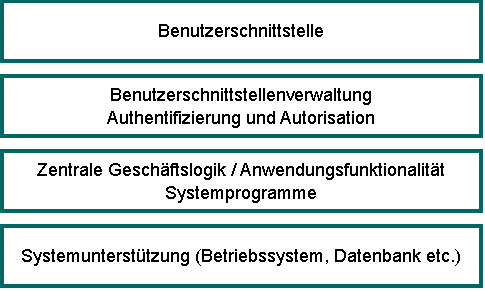
\includegraphics{Bilder/Kapitel-7/schichtenarchitektur_allgemein.pdf}
	\caption[Eine allgemeine Schichtenarchitektur]{Eine allgemeine Schichtenarchitektur, nach \cite[204]{som18}}
	\label{fig:schichtenarchitektur_allgemein}
\end{figure}

\vspace{\baselineskip} %%% für Druck

Abbildung~\ref{fig:schichtenarchitektur_allgemein} zeigt eine Schichtenarchitektur. Jede Schicht bildet einen logisch zusammenhängenden Zuständigkeitsbereich und setzt sich in der Regel aus mehreren Komponenten zusammen. In Systemen mit Benutzerinteraktion ist die oberste Schicht der Architektur die Benutzungsschnittstelle. Der Begriff Komponente im Zusammenhang mit Schichtenarchitektur benennt meist nicht das ganz „große“ Teilstück des Softwaresystems. Es handelt sich hier oft um die kleineren Einheiten, aus denen sich die großen Teilstücke zusammensetzen. Grundsätzlich abstrahiert das Modell der Schichtenarchitektur aber davon, was genau man in einem konkreten Softwareentwicklungsprojekt später als logische Einheit „Komponente“ 
\linebreak %%% für Druck
definiert.

Das grundsätzliche Prinzip bei einer Schichtenarchitektur ist, dass die Komponenten einer tieferliegenden Schicht die Dienstleister für die Komponenten der höheren Schichten sind, aber nicht umgekehrt. Das bedeutet, dass Komponenten in einer unteren Schicht für die Erbringung ihrer Funktionalität niemals auf die Funktionali\-täten von Komponenten einer höheren Schicht angewiesen sein dürfen. Abhängigkeiten einer Komponente kann es dann nur zu Komponenten unter ihr geben. Wenn dieses Prinzip eingehalten wird, kann es bei Veränderung oder Austausch einer bestimmten Komponente maximal Auswirkungen auf sie nutzende Komponenten in den darüber liegenden Schichten geben.

In einer sogenannten \textbf{strikten} Schichtenarchitektur dürfen Komponenten einer 
\linebreak %%% für Druck
Schicht nur Funktionalität von Komponenten der unmittelbar darunter liegenden Schicht verwenden. Das ist aber für viele Softwaresysteme nicht praktikabel und würde sich dort nur durch Codeduplizierung oder durch zusätzliche Komponenten, die rein für das „Durchleiten“ zuständig sind, realisieren lassen – beides widerspricht allgemeinen Entwurfsprinzipien. Daher werden Schichtenarchitekturen üblicherweise so eingesetzt, dass eine Komponente auch über mehrere Schichten hinweg auf Funktionalität einer in der Schichtenarchitektur unter ihr liegenden Komponente zugreifen kann.

Schichten sind lediglich logische Entwurfsgruppierungen von Komponenten des Softwaresystems. Sie werden bei der Implementierung üblicherweise nicht als ein eigenes „Konstrukt“ in den Programmcode übertragen. Im Programmcode direkt finden sich maximal die Komponenten (als Formen von Containerstrukturen wie zum Beispiel Packages in Java). Das zentrale Element im Programmcode sind die Klassen und diese sind aus Entwurfssicht gesehen die Bestandteile, aus denen sich die Komponenten zusammensetzen. Schichten bilden sich im Programmcode nur indirekt über die Aufruf-Abhängigkeiten der einzelnen Klassen untereinander ab.  

\begin{figure}[h!]
	\centering
	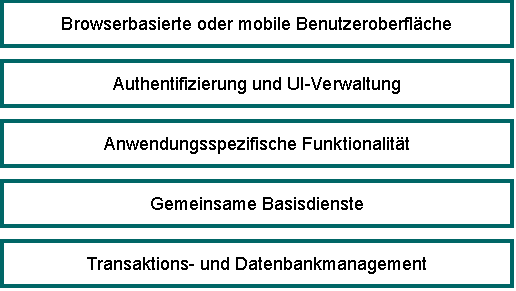
\includegraphics{Bilder/Kapitel-7/schichtenarchitektur_fuer_webbasierte_anwendungen.pdf}
	\caption[Eine Schichtenarchitektur für webbasierte Anwendungen]{Eine Schichtenarchitektur für webbasierte Anwendungen, nach \cite[108]{som20}}
	\label{fig:schichtenarchitektur_fuer_webbasierte_anwendungen}
\end{figure}

Eine Schichtenarchitektur muss nicht aus genau vier Schichten bestehen wie in \mbox{Abbildung}~\ref{fig:schichtenarchitektur_allgemein}. Die Anzahl der Schichten hängt vom konkret zu entwickelnden Software\-system und seinen geplanten Funktionalitäten ab. Für viele Anwendungs\-gebiete und Einsatzzwecke gibt es heute schon entsprechend angepasste detailliertere Schichtenarchitekturmodelle, die man gut als Ausgangspunkt für den Entwurf der eigenen Architektur verwenden kann. Abbildung~\ref{fig:schichtenarchitektur_fuer_webbasierte_anwendungen} zeigt eine verbreitete Schichtenarchitektur für webbasierte Softwareanwendungen. Bei \cite[108-113]{som20} finden Sie für diese Architektur eine detailliertere Beschreibung, welche Komponenten eines Softwaresystems man üblicherweise in welcher der Schichten platzieren würde, sowie die Anwendung dieser Architektur auf ein Fallbeispiel. Ein anderes Fallbeispiel mit vier Schichten zeigt \cite[214\psq]{som18}.
\subsubsection{Client-Server-Architekturen}
\label{sec:Kap-7.1.2.2}

Client-Server-Architekturen werden für webbasierte Softwaresysteme verwendet. Es gibt verschiedene Ausprägungen von Client-Server-Architekturen, aber das Grundprinzip ist immer dasselbe: Als Client dient der Computer bzw. das Mobilgerät des Nutzers, über den, zum Beispiel durch Browser oder App, mit der Benutzungs\-oberfläche interagiert werden kann. Die Softwareanwendung selber wird als eine Menge von Diensten organisiert, die auf einem oder mehreren entfernten Servern laufen. Die Clients der Nutzer greifen auf die benötigten Dienste zu und präsentieren dem Nutzer die Ergebnisse. Abbildung~\ref{fig:client_server_architektur} zeigt die Funktionsweise einer Client-Server-Architektur auf einer hohen Abstraktionsebene.

\vspace{\baselineskip} %%% für Druck
\vspace{\baselineskip} %%% für Druck

\begin{figure}[h!]
	\centering
	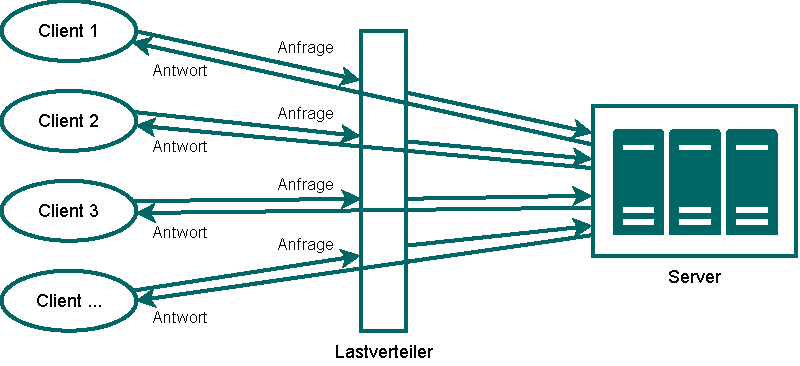
\includegraphics{Bilder/Kapitel-7/client_server_architektur.pdf}
	\caption[Client-Server-Architektur]{Client-Server-Architektur, nach \cite[114]{som20}}
	\label{fig:client_server_architektur}
\end{figure}

\vspace{\baselineskip} %%% für Druck

Auf Serverseite handelt es sich meistens nicht um einen einzigen Server, sondern um einen Serververbund, 
\marginline{Serververbund und Lastverteiler} 
an dem unterschiedlich viele Server beteiligt sein können. Client-Server-Architekturen sind darauf ausgerichtet, dass viele Clients unabhängig und ohne Kenntnis voneinander Anfragen an den Serververbund schicken können. Ein sogenannter Lastverteiler (engl. Load Balancer) verteilt die Anfragen an die beteiligten Server, um das Gesamtsystem auch bei großer Anzahl gleichzeitig eintreffender Anfragen performant zu halten. Der Lastverteiler selber ist entweder ein spezielles Hardwaregerät oder eine Load Balancing-Softwareanwendung auf einem Server. Im Unterschied zu den Servern im Serververbund ist dieser nicht an den zu erbringenden Diensten der eigentlichen Anwendungssoftware beteiligt, seine einzige Aufgabe besteht darin, die Anfragen geeignet zu verteilen.

Die Aufgabe der Clients 
\marginline{Aufgabengebiet der Clients} 
in Client-Server-Architekturen besteht mindestens darin, die Interaktion mit den Benutzern zu übernehmen. Zu Anfangszeiten von Client-Server-Architekturmodellen hatten die Clients häufig nur wenig Rechenkapazität. Ihre Tätigkeit war daher auf den Bereich der Nutzerinteraktion beschränkt, die gesamte Verarbeitung innerhalb des Softwaresystems fand auf dem Serververbund statt. Heute haben selbst Smartphones so viel Rechenkapazität, dass in vielen Software\-anwendungen die Clients neben der reinen Benutzerinteraktion auch für einen Teil der Datenverarbeitung zuständig sind. Das Prinzip der Zusammenarbeit von Client-Seite und Server-Seite ist aber nach wie vor dasselbe, nur die Arbeitsaufteilung unterscheidet sich.

\vspace{2mm} %%% für Druck

Client-Server-Architekturen und die zuvor vorgestellte Schichtenarchitektur \marginline{Bezug zur Schichten\-architektur} sind durchaus keine sich ausschließenden Architekturalternativen, sondern werden häufig in Kombination eingesetzt. Dafür wird innerhalb der Client-Server-Architektur das eigentliche Anwendungssystem nach Schichtenarchitektur organisiert. Client-Seite und Server-Seite sind dann jeweils für unterschiedliche Schichten verantwortlich. Abbildung~\ref{fig:schichtenarchitektur_fuer_client_server_architektur} zeigt eine Schichtenarchitektur, wie sie innerhalb von Client-Server-Ar\-chi\-tek\-tu\-ren vorkommen kann. Die Client-Seite ist für die Funktionalitäten der Präsentationsschicht zuständig, die Server-Seite für die drei anderen Schichten (sogenanntes Thin-Client-Modell). Die Client-Seite kann, wie im vorherigen Absatz beschrieben, aber auch zusätzlich für die Schicht Anwendungsverarbeitung zuständig sein, dann bleiben auf Server-Seite nur die beiden Schichten Datenbank und Datenverwaltung (Fat-Client-Modell). Man nennt diese Art der Architektur „zweischichtige Client-Server-Architektur“, wobei sich die „zwei“ auf die beiden Schichten Client und Server bezieht und nicht auf die Anzahl der Schichten der Anwendungssoftware.

\vspace{\baselineskip} %%% für Druck

\begin{figure}[h!]
	\centering
	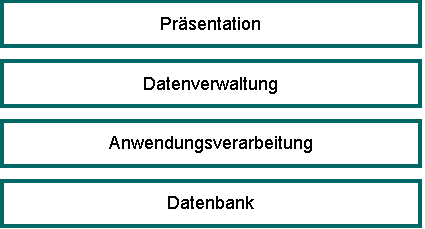
\includegraphics{Bilder/Kapitel-7/schichtenarchitektur_fuer_client_server_architektur.pdf}
	\vspace{2mm} %%% für Druck
	\caption[Schichtenarchitektur für eine Client-Server-Architektur]{Schichtenarchitektur für eine Client-Server-Architektur, nach \cite[564]{som18}}
	\label{fig:schichtenarchitektur_fuer_client_server_architektur}
\end{figure}

\vspace{\baselineskip} %%% für Druck

Alternativ zu den zweischichtigen Architekturen gibt es die mehrschichtigen Client-Server-Architekturen. Im Unterschied zu den zweischichtigen Architekturen wird hier die Serverseite noch weiter unterteilt. Abbildung~\ref{fig:client_server_architektur_mehrschichtig} zeigt eine heute übliche mehrschichtige Client-Server-Architektur mit Unterteilung in einen Webserver, einen Anwendungsserver und einen Datenbankserver. Alle drei Serverarten können natürlich auch mehrfach im Serververbund vorkommen, und zusätzlich können für die Skalierbarkeit der Anwendung wieder Lastverteilungsmechanismen vorhanden sein. Sehr ausführliche Informationen zu den hier beschriebenen und weiteren Client-Server-Architekturen finden Sie bei \cite[562-581]{som18}.

\begin{figure}[h!]
	\centering
	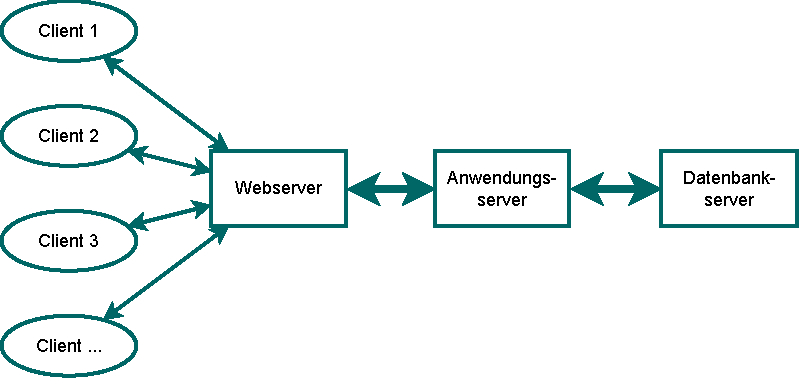
\includegraphics{Bilder/Kapitel-7/client_server_architektur_mehrschichtig.pdf}
	\caption[Mehrschichtige Client-Server-Architektur]{Mehrschichtige Client-Server-Architektur, nach \cite[117]{som20}}
	\label{fig:client_server_architektur_mehrschichtig}
\end{figure}

% Möglichkeit hier noch SOA zu thematisieren

\minisec{MVC-Muster}
\vspace{1mm} %%% für Druck

Innerhalb des Bereichs der Client-Server-Architekturmuster spielt ein weiteres 
\linebreak %%% für Druck
Muster eine wichtige Rolle, das sogenannte MVC-Muster.

MVC steht für Model-View-Controller. Zielsetzung des Musters ist die Entkopplung zwischen dem Modell (Daten und Geschäftslogik) einer Soft\-ware\-an\-wen\-dung und der Darstellung der Ausgabe. Dafür werden drei Komponenten Modell, Sicht und Programmsteuerung voneinander unabhängig gehalten und die notwendige Kommunikation zwischen ihnen findet nur über einen festgelegten Mechanismus statt. Das MVC-Muster wird sowohl als Architekturmuster – und dort nicht nur im Rahmen von Client-Server-Architekturen – als auch als Entwurfsmuster eingesetzt. Entwurfs\-muster operieren auf der Ebene der Klassen und Objekte, also auf einer deutlich niedrigeren Abstraktionsebene als Architekturmuster. Im Rahmen von Client-Server-Architekturen wird das MVC-Muster für die Organisation der Interaktion zwischen Client und Server verwendet. 

Es gibt das MVC-Muster aufgrund seiner verschiedenen Einsatzbereiche in verschiedenen Varianten. Etwas grundlegendere Unterschiede zwischen den Varianten bestehen einerseits in der Kommunikationsgestaltung zwischen Model und View und andererseits (bei Verwendung in Client-Server-Architekturen) in der Aufteilung der Komponentenzuständigkeit auf Client und Server. Die wesentliche Verfahrensweise des Musters ist aber gleich: Durch die Trennung von Model und View kann es mehrere Views zu einem Modell geben, die Daten des Modells damit in unterschiedlicher Weise dargestellt werden. Abbildung~\ref{fig:mvc_muster} zeigt eine Variante des MVC-Musters. 

\begin{figure}[h!]
	\centering
	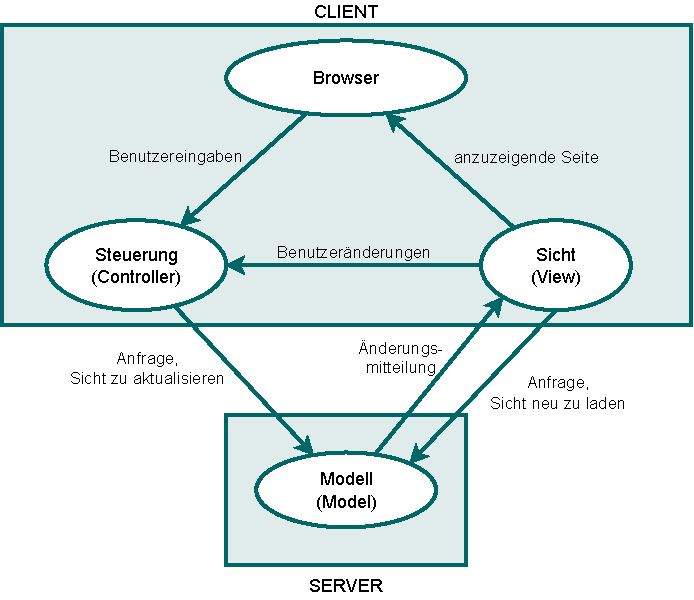
\includegraphics{Bilder/Kapitel-7/mvc_muster.pdf}
	\caption[Das MVC-Muster im Rahmen einer Client-Server-Architektur]{Das MVC-Muster im Rahmen einer Client-Server-Architektur, nach \cite[115]{som20}}
	\label{fig:mvc_muster}
\end{figure}

Auf jedem Client kann es mehrere Views geben, in denen die Daten unterschiedlich dargestellt sind. Die Views sind dabei unabhängig voneinander und zwar sowohl bezogen auf diesen einen Client als auch in Bezug zu den Views der anderen Clients. Jede View registriert sich bei dem Model. Das Model benachrichtigt alle bei ihm registrierten Clients, wenn sich Daten geändert haben, so dass die Views sich aktualisieren können. Benutzereingaben, die etwas am Modell ändern würden, werden über die Controller-Komponente des Musters behandelt.

% 7.2
\clearpage
\section{Entwurfsprinzipien}
\label{sec:Kap-7.2}

Im Prozess der Softwareentwicklung geht es auf verschiedenen Ebenen immer wieder darum, Komplexität zu reduzieren. \cite[19]{ous21} gibt eine sehr eingängige und praktische Definition von Komplexität: „Komplexität ist all das, was mit der Struktur eines Soft\-ware\-sys\-tems in Zusammenhang steht und dieses schwer verständlich und schwer anpassbar macht.“

Ein entscheidender Teil der Komplexität in einem Softwaresystem entsteht durch die Beziehungen zwischen den Komponenten. Je nachdem, auf welche Weise und wie stark Komponenten miteinander verbunden sind, wirken sich Änderungen an einer Komponente mehr oder weniger stark auf andere Komponenten aus. Ziel bei der Zerlegung der Systemfunktionalität in Komponenten – sei es als große Komponenten der Architektur, als kleinere Komponenten innerhalb dieser Architektur oder auf der niedrigen Ebene der Klassen – ist es, möglichst wenig Komplexität ins System zu bringen. Wenn alle Komponenten eines Systems völlig unabhängig voneinander wären, indem sich ihre Aufgabenbereiche nicht überschneiden und sie gar nicht miteinander verbunden wären, wäre man auf dem Weg der Komplexitäts\-reduktion schon recht weit – die reine Anzahl der Komponenten und die inhaltliche Komplexität der zu erfüllenden Aufgabe jeder Komponente bliebe natürlich noch. Ein solches System könnte aber fast immer seinen Zweck nicht erfüllen. Die im letzten Abschnitt vorgestellten Architekturmuster und die in diesem Abschnitt beschriebenen Entwurfsprinzipien sind Wege, sich einem komplexitätsreduzierten System, das aber trotzdem seinen Einsatzzweck erfüllt, anzunähern.

\minisec{Komponentenbeziehungen}

Komponenten können in unterschiedlichen Beziehungen zueinander stehen. Abbildung \ref{fig:komponentenbeziehungen} zeigt einige typische Komponentenbeziehungen in Softwaresystemen.

\vspace{\baselineskip} %%% für Druck

\begin{figure}[h!]
	\centering
	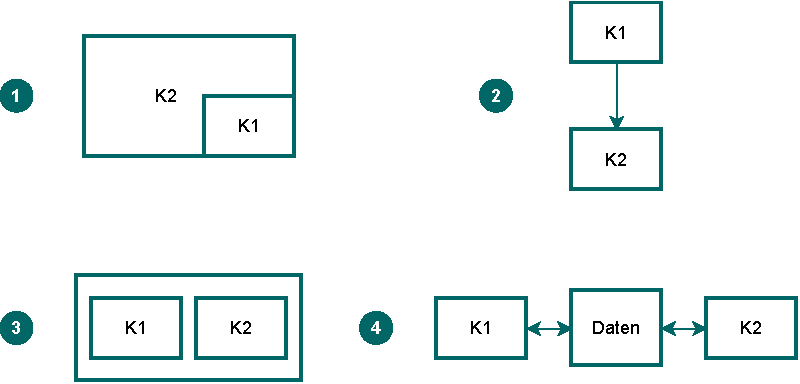
\includegraphics{Bilder/Kapitel-7/komponentenbeziehungen.pdf}
	\caption[Komponentenbeziehungen]{Komponentenbeziehungen, eigene Abbildung in Anlehnung an \cite[105]{som20}}
	\label{fig:komponentenbeziehungen}
\end{figure}

\vspace{\baselineskip} %%% für Druck

\begin{enumerate}
	\item \textbf{ist-Teil-von-Beziehung:} Eine Komponente (K1 in der Abbildung) kann Teil einer anderen Komponente sein (hier K2). So kann zum Beispiel eine bestimmte Operation Teil einer Klasse sein oder eine Klasse zur Zins\-berechnung Teil einer Komponente mit finanzmathematischen Funktionalitäten oder eine Komponente zur Anzeige der Benutzungsoberfläche Teil der Architektur\-komponente Benutzungsschnittstelle.
	\item \textbf{benutzt-Beziehung}: Eine Komponente (K1) verwendet die Funktionalität einer anderen Komponente (K2). Diese Beziehungsart findet man häufig. Auf der Ebene von Klassen und Objekten gehören sämtliche Aufrufe eines Objekts von Operationen anderer Objekte dazu.
	\item \textbf{ist-zusammen-mit-Beziehung:} Zwei Komponenten (K1 und K2) sind in derselben übergeordneten Struktur (das äußere Rechteck) verortet. Auf 
	\linebreak %%% für Druck
	Architekturebene trifft das zum Beispiel auf Komponenten zu, die sich in derselben Schicht einer Schichtenarchitektur befinden.
	\item \textbf{teilt-Daten-mit-Beziehung} Eine Komponente teilt Daten mit einer anderen Komponente. Hier könnte man noch weiter unterscheiden, wie genau dieses Teilen von Daten aussieht, zum Beispiel ob beide Komponenten auf dieselbe Datenbasis zugreifen (so ist es in der Abbildung) oder ob es einen Datenfluss zwischen ihnen gibt etc.
\end{enumerate}

In allen Fällen können die Abhängigkeiten zwischen den Komponenten dazu führen, dass Änderungen bei einer der beiden Komponenten Änderungen an der anderen Komponente nach sich ziehen. Genau das versucht man in der Softwareentwicklung zu vermeiden. Bewährte Entwurfsprinzipien zeigen Strategien auf, wie man trotz dieser Arten von Abhängigkeiten zwischen den Komponenten den Änderungsbedarf an verbundenen Komponenten minimiert.

\subsection{Entwurfsprinzipien zur Schnittstellengestaltung}
\label{sec:Kap-7.2.1}

Wir beginnen auf der niedrigen Abstraktionsebene der Klassen und Objekte: Ein zentrales Charakteristikum der Objektorientierung ist die Kapselung von Daten und Operationen innerhalb eines Objekts. Auf den Daten eines Objekts arbeiten bei konsequenter Einhaltung des Prinzips der Kapselung nur seine eigenen Operationen. Ein Entwurfsprinzip, das die Einhaltung der Kapselung unterstützen soll, ist das \textit{Geheimnisprinzip} 
\marginline{Geheimnis\-prinzip} 
(engl. Information Hiding). Es besagt, dass ein Objekt nur genau den Teil seiner Funktionalität nach außen für Objekte anderer Klassen zur Verfügung stellt, den diese benötigen. Auf Klassenebene bedeutet das, dass die Implemen\-tierungs\-details einer Klasse vor anderen Klassen verborgen werden, das heißt, dass die Programmierung der Funktionalitäten in den anderen Klassen nicht davon abhängig sein darf, wie der Programmcode dieser einen Klasse aussieht. So sollen zum Beispiel der konkrete Programmcode der Operationen, verwendete Daten\-strukturen, aber auch die Attribute einer Klasse anderen Klassen nicht bekannt sein. Zudem brauchen nur die Operationen außen bekannt sein, die auch außerhalb der Klasse benötigt werden. Operationen, die zum Beispiel interne Berechnungen durchführen oder verwendet werden, um eine komplexere Funktionalität auf mehrere Operationen aufzuteilen, können verborgen sein. 

Den Teil einer Klasse, der nach außen sichtbar ist, nennt man seine \textit{Schnittstelle}. Die Schnittstelle enthält all das, was Objekte anderer Klassen kennen müssen, um die Funktionalität des Objekts dieser Klasse verwenden zu können. \marginline{Schnittstelle} Die Schnittstelle der Klasse gibt Auskunft darüber, \textbf{was} die Klasse tut, aber nicht \textbf{wie} sie es tut. Objekte anderer Klassen rufen über die Schnittstelle die Dienstleistungen (Funktionalitäten) der Klasse auf.

\vspace{-0.1mm} %%% für Druck

Wir gehen jetzt eine Ebene höher, abstrahieren von einzelnen Klassen und sprechen allgemeiner von Komponenten. Eine Komponente kann dabei einer einzelnen Klasse entsprechen, aber ebenso gut auch eine logisch zusammengehörige Menge mehrerer Klassen sein. Die Schnittstelle einer Komponente macht genau das Gleiche, was die Schnittstelle der Klasse von eben getan hat: sie gibt Auskunft darüber, was die Komponente tut, damit andere Komponenten über diese Schnittstelle die benötigten Dienstleistungen von ihr erhalten können. Noch eine Ebene höher bei den Architektur\-komponenten haben wir das gleiche Prinzip: Die Komponente, zum Beispiel eine der Schichten einer Schichtenarchitektur, gibt über ihre Schnittstelle Auskunft über ihre Dienstleistungen. Im Unterschied zur niedrigen Ebene der Klassen wendet man das Geheimnisprinzip auf den höheren Ebenen oft nicht ganz so strikt an, verbirgt also nicht immer die komplette innere Struktur der Komponente (aus welchen Teilkomponenten besteht sie, wie verteilen sich ihre Funktionalitäten auf ihre Teile etc.), da auch zu viel Abstraktion die Komplexität eines Systems erhöhen kann. 

\vspace{-0.1mm} %%% für Druck

Alle anderen Entwurfsprinzipien, die sich mit Schnittstellen von Komponenten beschäftigen, konkretisieren das Geheimnisprinzip, indem sie spezifizieren, wie die Schnittstelle der Komponente aussehen soll und damit festlegen, was und wie viel und in welcher Form nach außen sichtbar sein soll. 

\vspace{-0.1mm} %%% für Druck

Schnittstellen sollten sich möglichst nicht verändern, weil sonst alle Komponenten, die diese Schnittstelle verwenden, ebenfalls geändert werden müssten. Im besten Fall betrifft das nur den Aufrufmechanismus für die Schnittstelle in den verwendenden Komponenten, aber selbst das kann aufwändig sein und ist in jedem Fall fehleranfällig. \marginline{stabile Schnittstellen} Einen echten Namen hat diese kleine Regel nicht, Sie finden sie unter Schlagworten wie „stabile Schnittstellen“ oder „feste Schnittstellen“ in der Literatur.

\vspace{-0.1mm} %%% für Druck

Ein echtes Entwurfsprinzip ist \textit{Program to Interfaces}, 
\marginline{Program to Interfaces} 
auf Deutsch „Programmiere gegen Schnittstellen“, auch unter der Bezeichnung „Trennung der Schnittstelle von der Programmierung“ zu finden. Insbesondere in der letzten Übersetzung (und in manchen Beschreibungen in der Literatur) wirkt es zunächst wie altes Geheimnisprinzip in neuen Schläuchen. Das Prinzip geht aber darüber hinaus. Etwas vereinfacht ausgedrückt: Das Geheimnisprinzip sagt, \textbf{was} von der Komponente verborgen bleiben soll. Das Program~to Interfaces-Prinzip sagt, \textbf{dass} die Komponente verborgen bleiben soll. Das Prinzip wird üblicherweise auf der niedrigen Ebene der Klassen kommuniziert, ließe sich von der Idee her aber auch auf die höheren Ebenen übertragen. 

\vspace{-0.1mm} %%% für Druck

Die Idee des Program to Interfaces-Prinzips ist, dass man die Implementierung einer Komponente und die Schnittstelle, die man Dienstnutzer-Komponenten zur Verfügung stellt, als zwei komplett getrennte Aspekte betrachtet und nicht als zwei Teilstücke derselben Komponente. Ihre Verbindung ist, dass die Schnittstelle Funktionalität der Art anbietet, wie sie die Implementierung der Komponente erbringen kann. Dem Dienstnutzer, der die Schnittstelle verwendet, bleibt verborgen, welche Komponente genau die Dienstleistung erbringt. Genau genommen ist diese Schnittstelle dann auch nicht mehr die Schnittstelle einer \textbf{bestimmten} Komponente, sondern die einer Art „Komponenten-Verwandtschaft“, nämlich alle potenziellen Komponenten, die genau die in der Schnittstelle spezifizierte Funktionalität erbringen könnten.
 
Der Sinn hinter dem Program to Interfaces-Prinzip ist Austauschbarkeit. Indem man Schnittstelle und Implementierung so voneinander separiert, kann man die konkrete Implementierung (also die ganze Komponente) wegnehmen und durch eine andere Komponente mit gleicher Wirkungsweise ersetzen, ohne dass die Dienstnutzer davon etwas merken. 

Ein anderes Entwurfsprinzip, das sich mit Schnittstellen befasst, ist das 
\marginline{Interface Segregation Principle} 
\textit{Interface \mbox{Segregation} Principle}. Es konkretisiert das Geheimnisprinzip, indem aus „Die 
\linebreak %%% für Druck
Schnittstelle der Komponente enthält nur das, was die Dienstnutzer-Komponenten brauchen“ ein „Die Schnittstelle für eine Dienstnutzer-Komponente enthält nur genau das, was diese Komponente braucht“ wird. Und das läuft dann darauf hinaus, dass es zu einer Komponente mehrere Schnittstellen gibt, von denen jede für eine andere Dienstnutzerrolle gedacht ist und entsprechend nur die Funktionalität zur Verfügung stellt, die genau diese Rolle benötigt. Analogie aus einem ganz anderen Bereich: das ist ein wenig ähnlich zur Idee hinter den User Stories in der Anforderungs\-ermittlung.

Der Sinn hinter dem Prinzip ist, dass von Änderungen an einer Schnittstelle möglichst wenige Dienstnutzerrollen betroffen sind, nämlich nur diejenigen, die die geänderte Funktionalität überhaupt verwenden. Wenn man stattdessen nur die eine Schnittstelle für alle Dienstnutzer-Komponenten verwenden würde, müssten eventuell auch solche Dienstnutzer-Komponenten verändert werden, die den geänderten Teil der Schnittstelle gar nicht verwenden – mindestens müsste geprüft werden, \textbf{ob} sich etwas für sie ändert.

Mit Änderungen an Schnittstellen sollte man zwar insgesamt vorsichtig sein, doch insbesondere wenn ein Softwareprodukt auf eine neue Version umgestellt wird oder andere Dienstnutzer-Komponenten mit zusätzlichen Bedürfnissen hinzukommen, lassen sie sich nicht immer vermeiden.
\vspace{-2mm} %%% für Druck

\subsection{Entwurfsprinzipien zu Komponentenzuständigkeiten}
\label{sec:Kap-7.2.2}

\vspace{-2mm} %%% für Druck

Im vorherigen Abschnitt haben wir Entwurfsprinzipien betrachtet, die die Gestaltung von Schnittstellen betrachten und bei denen somit die Zusammenarbeit zwischen den Komponenten im Fokus steht. Ebenso wichtig für eine möglichst geringe Komplexität des zukünftigen Softwaresystems ist eine geeignete Aufteilung der zu erbringenden Aufgaben auf die Komponenten. Hier geht es also um Zuständigkeiten.

Entwurfsprinzipien in diesem Bereich gehen von der Prämisse aus, dass es -- euphemistisch ausgedrückt -- suboptimal ist, wenn es keine klaren Zuständigkeiten gibt. Dies ist durchaus mit menschlichen Arbeitszusammenhängen vergleichbar: Wenn jeder irgendwie so ein bisschen für alles zuständig ist, aber nie komplett für alles aus einem Bereich, jeder etwas andere Arbeitsprozesse bevorzugt und man nicht sicher weiß, ob sich jemand anderes schon gekümmert hat \ldots, dann gibt es irgendwann Chaos. Und je mehr Menschen beteiligt sind, desto wahrscheinlicher und desto schneller befindet man sich in dieser Situation. Chaos auf der Ebene von Softwaresystemen und Komponenten bedeutet Komplexität, die nicht mehr beherrscht wird. Die Folgen sind Systeme, die nicht wartbar sind, nicht reproduzierbare Fehler verursachen, eine undurchschaubare Benutzungsoberfläche haben, inkonsistente Daten produzieren etc.

\vspace{0.8mm} %%% für Druck

Ein bekanntes Entwurfsprinzip zur Vermeidung einer solchen Situation ist 
\marginline{Separation of Concerns}
\textit{Sepa\-ration of Concerns (SoC)}, in deutschen Übersetzungen als Trennung der Belange/""Anliegen bezeichnet. Das SoC-Prinzip wird häufig mit der Ebene der Software\-architektur assoziiert. Es funktioniert durchaus auch auf niedrigeren Komponenten\-ebenen und wird auch dort verwendet, nur nennt man es dann nicht immer SoC (\su). 

\vspace{0.8mm} %%% für Druck

Die Grundaussage ist, dass getrennte Anliegen von getrennten Komponenten behandelt werden sollen. SoC beinhaltet ebenfalls, dass ein bestimmtes Anliegen nur durch eine Komponente repräsentiert wird und nicht über mehrere Komponenten verstreut sein soll. Das führt zu einer 1-zu-1-Beziehung zwischen Anliegen und Komponente.

\vspace{0.8mm} %%% für Druck

Beispiele für Anliegen auf der Ebene der Architektur sind Benutzerinteraktion oder Datenbankmanagement. Nach dem SoC-Prinzip sollte es bei diesen Beispielen keine Komponente geben, die gleichzeitig Aufgaben aus dem Bereich der Benutzer\-inter\-aktion und Aufgaben aus dem Bereich Datenbankmanagement übernimmt. Gleichzeitig sollen alle Aufgaben aus dem jeweiligen Bereich in derselben Komponente verortet sein. Für die beiden Beispiele ist das genau das, was die Schichtenarchitektur aus Abschnitt~\ref{sec:Kap-7.1.2.1} berücksichtigt: Die Benutzerinteraktion ist in einer Komponente, nämlich in der obersten Schicht der Architektur, und das Datenbankmanagement ist in einer anderen Komponente (eine der unteren Schichten). 

\vspace{0.8mm} %%% für Druck

Es gibt aber architektonische Anliegen, das klassische Beispiel ist Authentifizierung, die in mehreren Schichten relevant sind und für die man dementsprechend in mehreren Schichten Komponenten vorsehen würde. Bei Anwendung des SoC-Prinzips müsste sich der gesamte Programmcode für die Authentifizierungsaufgaben der verschiedenen Ebenen aber in einer Komponente befinden. Das ließe sich durchaus lösen, indem eine solche Authentifizierungskomponente so weit unten in der Schichten\-architektur platziert würde, dass sich alle Dienstnutzer-Komponenten, die irgendeine Art von Authentifizierungsfunktionalität benötigen, in Schichten über ihr befinden. Der enorme Nachteil dieser Lösung ist ein deutlich erhöhter Kommunikationsbedarf zwischen Komponenten, und das häufig sogar über mehrere Schichten. 

\vspace{0.8mm} %%% für Druck

Für solche Anliegen, die bereichsübergreifend sind und daher in der Architektur auf mehreren Schichten berücksichtigt werden müssen (man nennt sie 
\marginline{Cross-Cutting Concerns} 
Cross-Cutting Concerns), verletzt man teilweise bewusst das SoC-Prinzip. Den umgekehrten Weg geht übrigens die sogenannte „Aspektorientierte Programmierung“. Sie stellt das SoC-Prinzip für solche Cross-Cutting Concerns in den Vordergrund und verletzt dafür bewusst das objekt\-orientierte Kapselungsprinzip. Ob aspektorientierte Programmierung ein eigenes Programmierparadigma ist oder nur eine „Erweiterung“ der objektorientierten Programmierung, wird nicht einheitlich gesehen. Ausführliche Informationen zur aspektorientierten Programmierung und wie man sie im Rahmen der objektorientierten Programmierung einsetzen kann, finden Sie bei \cite[533-578]{lah18}. 

Das Separation of Concerns-Prinzip ist eigentlich nicht spezifisch auf die Ebene der Softwarearchitektur ausgerichtet. Auch getrennte Komponenten für Datenhaltung und Datendarstellung, für Berechnungen und Anzeige der Ergebnisse dieser Berechnungen oder für die Gestaltung von Inhaltsbereich und Navigationsbereich einer Website ist angewendetes Separation of Concerns. Wenn wir auf eine ganz niedrige Abstraktionsebene gehen und Operationen als Komponenten einer Klasse ansehen, dann könnte man sogar die Aufteilung in Attributwert-lesende Operationen (get-Operationen) und Attributwert-schreibende Operationen (set-Operationen) als dem SoC-Prinzip folgend ansehen. 

\vspace{1.8mm} %%% für Druck

Bei all den Komponentenbegriffen unterhalb der Ebene der Softwarearchitektur spricht man selten explizit davon, dass man das SoC-Prinzip berücksichtigt. \mbox{Eventuell} hat das auch damit zu tun, dass auf diesen Ebenen mit dem Single Responsibility Principle ein eng verwandtes Prinzip recht bekannt ist.

\vspace{1.8mm} %%% für Druck

Das \textit{Single Responsibility Principle (SRP)}
\marginline{Single Responsibility Principle}
fokussiert auf die Zuständigkeiten der einzelnen Klassen innerhalb des Programms. Sie können aber auch hier den Begriff Klasse durch Komponente ersetzen und das Prinzip eine Ebene höher anwenden. Das SRP besagt, dass jede Klasse nur genau eine Verantwortung übernehmen soll. Gleichzeitig soll jede Verantwortung genau einer Klasse zugeordnet werden. Genau wie beim Separation of Concerns-Prinzip haben wir hier wieder eine 1-zu-1-Beziehung.
 
\vspace{1.8mm} %%% für Druck

In der Literatur findet sich für die Aussage des Prinzips auch die Formulierung „nur eine Aufgabe haben“ oder die Formulierung, dass jede Klasse nur aus genau einem Grund geändert werden soll – die Unterschiedlichkeit ist in der Genese des Prinzips begründet (s. \cite[406]{bro21}). Alle Formulierungen meinen aber dasselbe: Eine Klasse ist für eine bestimmte Aufgabe verantwortlich und nur wenn sich an dieser Aufgabe etwas ändert, ist das ein Grund die Klasse anzupassen. Wenn man andere Gründe findet, die Klasse zu ändern, dann bedeutet das, dass die Klasse entgegen des Prinzips eben nicht nur für die eine Aufgabe, sondern offensichtlich auch noch für etwas anderes zuständig war. 

\vspace{1.8mm} %%% für Druck

Was soll man sich jetzt unter einer solchen \textbf{Aufgabe} vorstellen? Im Grunde geht es ganz einfach um die Anforderungen an das Softwaresystem. Nach dem SRP-Prinzip soll jede einzelne Klasse die Verantwortung für einen klar definierten Teil der Anforderungen übernehmen und deren Umsetzung gewährleisten. Gleichzeitig darf keine andere Klasse für die Umsetzung derselben Anforderungen zuständig sein. Und außerdem dürfen am Ende auch keine Anforderungen übrig bleiben, weil keine der Klassen Verantwortung für sie hat. Die Aufgabe einer einzelnen Klasse besteht also aus einer oder mehreren zusammengehörigen Anforderungen. Der einzige Grund die Klasse zu verändern, ist, dass sich die Anforderungen, für die die Klasse zuständig ist, geändert haben. 

\vspace{1.8mm} %%% für Druck

Bleibt noch die Frage, nach welchen Gesichtspunkten die Anforderungen aufgeteilt werden. Meine fünfzehn Anforderungen willkürlich auf vier Klassen zu verteilen, ist sicher nicht zielführend in Richtung Komplexitätsvermeidung. Hier arbeitet SRP nach dem Separation of Concerns-Prinzip: logisch getrennte Anliegen (hier Anforderungen) werden in getrennten Klassen behandelt; Anforderungen, die logisch zusammengehören, dementsprechend in derselben Klasse behandelt. Für diejenigen von Ihnen, denen der Begriff Kohäsion schon etwas sagt: hohe Kohäsion der Klasse ist das Kriterium, anhand dessen beim SRP die Aufgabe einer Klasse spezifiziert wird. Wir werden das Thema Kohäsion in Lektion~6 behandeln.

\vspace{2mm} %%% für Druck

Was unterscheidet SRP und SoC 
\marginline{SRP und SoC} 
oder ist es dasselbe? Das ist eine durchaus uneinheitlich beantwortete Frage. Ein Unterschied ist sicherlich der Blickwinkel. Das Separation of Concerns-Prinzip beginnt bei den Aufgaben, die insgesamt zu tun sind, trennt alles, was logisch nicht zusammengehört und bündelt das logisch Zusammengehörige in derselben Komponente. Das Single Responsibility-Prinzip beginnt bei der Komponente und spezifiziert anhand des logischen Zusammenhangs, welchen Teil der Gesamtaufgaben diese Komponente übernehmen soll. Das tut es für alle Komponenten. SoC fokussiert also auf die Aufgaben, SRP auf die Komponenten. Allerdings ist das Ergebnis am Ende dasselbe: eine Menge an Komponenten, jede von ihnen in sich logisch zusammenhängend und nach außen aufgrund der logisch unterschiedlichen Anliegen von den anderen Komponenten getrennt. Auch die Argumen\-tation SoC arbeitet auf der Ebene der Softwarearchitektur und SRP auf der Ebene der Klassen und damit sind Anliegen im Sinne von SoC etwas viel Größeres als das, was SRP als Aufgabe betrachtet, ist sicherlich nicht falsch -- man macht es oft so -- aber wie oben mehrfach erwähnt, sind bei beiden die Grenzen fließend. Wir schließen uns hier der Meinung an, dass SRP eine bestimmte Ausgestaltung (Ausprägung, Version) von SoC ist, die vorwiegend auf Ebene der Klassen operiert und die Verantwortung der einzelnen Klasse in den Fokus nimmt anstelle der Gesamtheit der Aufgaben. 

\vspace{2mm} %%% für Druck

\subsection{Fazit}
\label{sec:Kap-7.2.3}

Neben übergreifenderen Entwurfsprinzipien, wie wir sie in den beiden vorherigen Abschnitten vorgestellt haben, gibt es auch viele kleinere Prinzipien wie „Codeduplizierung vermeiden“ oder „zukünftige Erweiterungen“ mitdenken. Auf einige davon treffen Sie noch im folgenden Kapitel, wenn wir unseren Blickwinkel ganz auf die niedrige Komponentenebene der Klassen richten. Auf andere, die sehr Programmcode-nah sind, wie den Umgang mit Sichtbarkeiten in einer Klasse, gehen wir in Lektion~6 ein.

\vspace{2mm} %%% für Druck
  
Allen Entwurfsprinzipien -- den übergreifenden und den kleinen, den abstrakten und den Programmcode-nahen -- ist gemein, dass sie eine Idealvorstellung betrachten, wie eine Komponente sein muss. Wir hatten in Abschnitt~\ref{sec:Kap-7.1} eine Komponente als Einheit zusammengehöriger Funktionalität definiert. Hier verfeinern wir diese Definition entsprechend dieser Idealvorstellungen (basierend auf \cite[309f.]{bro21}). Eine Komponente

\begin{itemize}
	\setlength{\itemsep}{2mm} %%% für Druck
	\item kapselt Teilfunktionalität des Gesamtsystems,
	\item bietet ihre Dienstleistungen über eine oder mehrere klar spezifizierte Schnittstellen anderen Komponenten an,
	\item kann Abhängigkeiten zu den Diensten anderer Komponenten haben. Diese Abhängigkeiten müssen dann aber klar spezifiziert sein,
	\item kann unabhängig von anderen Komponenten entwickelt werden,
	\item kann grundsätzlich auch unabhängig von anderen Komponenten eingesetzt werden, erbringt ihre volle Funktionalität aber aufgrund eventueller Abhängig\-keiten zu den Diensten anderer Komponenten erst im Zusammenwirken,
	\item kann mit anderen Komponenten zu größeren Einheiten kombiniert werden. Die Komponente selber ändert sich dabei nicht.
\end{itemize} 




% 7.3
\clearpage
\section{Kommentierte Literatur}
\label{sec:Kap-7.3}


\sttpKommLitItem{Sommerville}{2020}{Modernes Software-Engineering}{som20}{}{}
{Kapitel 4 behandelt das Thema Softwarearchitektur mit Schwerpunkt auf Einflussfaktoren und Architekturmustern. Dieses Kapitel haben wir als Grundlage für die Themen in Abschnitt~\ref{sec:Kap-7.1} verwendet. Deshalb werden Sie hier fündig, wenn Sie zu diesen Themen noch weiter ins Detail gehen möchten. Entwurfsprinzipien werden nur am Rande im Zusammenhang mit Cross-Cutting Concerns behandelt.}

\sttpKommLitItem{Lahres/Raýman/Strich}{2018}{Objektorientierte Programmierung}{lah18}{Bilder/Buchcover/Buchcover_Lahres_Rayman_Strich.png}{}
{Kapitel 3 stellt Entwurfsprinzipien der objektorientierten Programmierung vor. 
\linebreak %%% für Druck
Außer dem Interface Segregation Principle kommen alle im Lerntext behandelten Prinzipien vor, teilweise mit etwas anderen Namen. Zudem werden weitere Entwurfs\-prinzipien thematisiert. Die Darstellung der Prinzipien ist gut zu lesen, weil viel mit Beispielen und mit Analogien aus der Realwelt gearbeitet wird.}

\sttpKommLitItem{Broy/Kuhrmann}{2021}{Einführung in die Softwaretechnik}{bro21}{}{}
{Sehr ausführliche Darstellung der Prozesse des Softwareengineering. Dem Prozess Entwurf sind die Kapitel acht bis zehn gewidmet, insgesamt fast 120 Seiten. Einen großen Stellenwert bekommt dort auch das Thema Wiederverwendung bewährten Wissens. Innerhalb von Kapitel 8 und von Kapitel 10 befinden sich kurze, gut verständliche Zusammenfassungen vieler verschiedener Entwurfsprinzipien (S. 329-341 und 405-417).}

\sttpKommLitItem{Ousterhout}{2021}{Prinzipien des Softwaredesigns}{ous21}{}{}
{Sehr auf den praktischen Einsatz orientierte Darstellung zahlreicher Entwurfs-
\linebreak %%% für Druck
prinzipien, die auf die niedrige Abstraktionsebene der Klassen fokussiert. Eher kein Nachschlagewerk für einzelne Prinzipien, sondern auf sequentielles Lesen ausgerichtet. Hilfreich sind die guten Zusammenfassungen am Ende jedes Kapitels.}

\sttpKommLitItem{Sommerville}{2018}{Software Engineering}{som18}{Bilder/Buchcover/Buchcover_Sommerville.jpg}{}
{Im Überblickskapitel über Softwareprozesse (Kap. 2) befindet sich ein kurzer, sehr gut zusammenfassender Abschnitt über den Ablauf und die Aufgaben im Software\-engineering-Prozess Entwurf (S. 67-69). Kapitel 6 befasst sich ausführlich mit dem Thema Softwarearchitektur. Hier finden Sie auch noch weitere Architekturmuster.}


